\documentclass[11pt]{amsart}

\usepackage[letterpaper,left=125pt,right=125pt]{geometry}
\usepackage{caption}
\usepackage{subcaption}
\usepackage{graphicx}
\usepackage{mwe}
% ^^^^^^^^^^^^^^^^^^^^^^^^^^^^^^^^^^^^^^^^^^^^^^^^^^^^^^^^^^^^^^^^^
% DO NOT change anything above this line! 
% (We need standard margins and type size.)
% In particular, don't include your own "geometry" settings further down.



%%%%%%%%%%%%%%%%%%%%%%%%%%%%%%%%%%%%%%%%%%%%%
% The following part of the preamble sets up packages, theorems, and shortcuts; 
% you can edit it, but you won't need to change much.

%% Load Packages:

\usepackage{blkarray}

\usepackage[english]{babel}
\usepackage {amsmath}  % provides lots--- e.g. equations, matrices, definition by cases
\usepackage{amssymb}  % provides common mathematical symbols
\usepackage{amsfonts}
\usepackage{amsthm}     %provides \newtheorem, \theoremstyle, \begin{proof}...\end{proof}
\usepackage{graphicx}  % allows importation of graphics files

\usepackage[colorlinks,linkcolor=blue,citecolor=blue,urlcolor=blue]{hyperref} % typesets URLS and clickable cross-references and links
%\usepackage{hyperref} % if you don't want colored links, just use the simpler command

\usepackage{float}

%\usepackage[backend=bibtex]{biblatex} % bibliography support
%\addbibresource{sample.bib} % CHANGE this to the name of your BibTeX database file (see instructions below)

%% Environments for theorems, etc.. 

% You can add your own theorem-like environments, see https://en.wikibooks.org/wiki/LaTeX/Theorems
% The basic format is \newtheorem{name}{display-text}[numbered-within] or \newtheorem{name}[numbered-like]{display-text}

\theoremstyle{theorem} % set the style for the following theorems

\newtheorem{thm}{Theorem}[section] %\newtheorem{name}{display-text}[numbered-within]

\newtheorem{lem}[thm]{Lemma} %\newtheorem{name}[numbered-like]{display-text}
\newtheorem{cor}[thm]{Corollary}
\newtheorem{prop}[thm]{Proposition}
\newtheorem{alg}[thm]{Algorithm}

\theoremstyle{definition}                  % switch to a different style
\newtheorem{defn}[thm]{Definition}
\newtheorem{conj}[thm]{Conjecture}


\theoremstyle{example}                       % another style
\newtheorem{prob}[thm]{Problem}


\theoremstyle{remark}                       % another style
\newtheorem{exmp}[thm]{Example}  % (note:the "example" style is not really good for long examples-- typesets them in italics!)
\newtheorem{rem}[thm]{Remark}
\newtheorem{claim}[thm]{Claim}  
\renewcommand{\theclaim}{}

%% If you use numbered equations in a long document, it is preferred to number
% as (x.y), where x is section number, y is equation number

\numberwithin{equation}{section}


%% Common typesetting for common mathematical objects

\newcommand{\R}{\mathbb{R}}
\newcommand{\Q}{\mathbb{Q}}
\newcommand{\N}{\mathbb{N}}
\newcommand{\Z}{\mathbb{Z}}
\DeclareMathOperator{\rank}{rank}
\DeclareMathOperator{\dimension}{dim}

\usepackage{cite}

%%%%%%%%%%%%%%%%%%%%%%%%%%%%%%%%%%%%%%
% BEGIN: You'll _need_ to edit everything below....


%  Your data for title, author, etc.

\title{Markov Chain Monte Carlo Simulation with Applications} % here, the command format is  \title[Abbreviated Title for Header]{Full Title}. But if your title is short, simply use \title{Full Title}
\thanks{This document is a senior thesis submitted to the Mathematics and Statistics Department of Haverford College in partial fulfillment of the requirements for a major in Mathematics. Special thanks to my advisor Weiwen Miao and to Lynne Butler for help and moral support.} % REQUIRED: don't change this line
\author{Isaiah Kriegman}
\date{2019-10-29} % don't forget to update the date!

\begin{document}

\begin{abstract}
    In this paper we outline the basic theory and practice of Markov Chain Monte Carlo (MCMC) simulation. The paper serves to assist readers in carrying out their own experiments. In the section on Markov chains, we define terms and prove basic theorems that provide the later foundation for our simulations. We give a brief general overview of Bayesian modeling to help describe applications. We cover the two biggest algorithms, the Metropolis-Hastings algorithm and Gibbs sampling, along with basic demonstrations. We provide illustrative figures and R code to explain these demonstrations.
\end{abstract}

\maketitle % Actually typeset the title, author, etc.

\section{Introduction}

Markov Chain Monte Carlo (MCMC) simulation refers to several techniques for sampling from unknown or difficult to sample from probability distributions. The basic concept is that with a clever transition rule, a Markov chain can be used to sample from a complicated distribution. This has led to a so-called `revolution' in the sciences, with computational papers in many fields opting to use it (see \cite{rev}). This paper will exposit the background and content of the most popular MCMC methods. The methods and diagnostic tools for carrying out real world experiments will be covered as well. The final chapters will attempt to go beyond theory and look at the developments that have enabled MCMC simulation to become commonplace in the sciences, as well as conducting an original investigation. We begin with a background on the methamtics of Markov chains.

\section{Markov Chains and Background}

\subsection{Markov Chains}

Markov Chains were introduced by Andrey Markov in 1906 in order to prove that the weak law of large numbers does not require strict independence of random variables. In particular he conducted an experiment where he recorded all of the two letter bigrams in a Pushkin's \emph{Eugene Onegin} to demonstrate his property \cite{pierre}. Whether he intended it or not, Markov Chains have since become a powerful modeling tool used across machine learning and Bayesian statistics. In this section we cover the basic properties of Markov chains and develop the theory necessary to understanding MCMC simulation.

The following definitions give explanations for Markov Chains on discrete state spaces. The definitions here come from chapter 11 of \emph{Markov chains} from Introduction to Probability by Blitzstein and Hwang \cite{blitzstein}.

\begin{defn}[{Markov Chain, \cite[p.~459]{blitzstein}}]
    A sequence of random variables $X_0, X_1, ...$ defined on a finite or countable \emph{state space} $\{1, 2, ... , M\}$ or $\{1, 2, ...\}$ is called a \emph{Markov chain} if for all $n\geq0$
    \[P(X_{n+1}=j|X_n=i_n, X_{n-1}=i_{n-1}, ... , X_0=i_0)=P(X_{n+1}=j|X_n=i).\] 
    
    This condition is called the \emph{Markov property}.
    
\end{defn}

The Markov property states that the probability of transitioning from state $i$ to $j$ when moving from $X_n$ to $X_{n+1}$ is \emph{only} dependent on the fact that $X_n=i$. If we consider the variables in the chain to be steps in time, with $n$ representing the step number, then all of the steps before $n$ do not tell us anything about the distribution of $X_{n+1}$.

\begin{defn}[{Transition matrix, \cite[p.460]{blitzstein}}]
    If $X_0, X_1, ...$ is a Markov chain on a countable state space $\chi=\{1, 2, ...\}$, then the matrix $Q$ with cells $q_{ij}=P(X_{n+1}=j|X_n=i)$ is called the \emph{transition matrix} of the chain.
\end{defn}

Note that if the state space is finite with $M$ states, then the dimensions of $Q$ are $M \times M$. If the state space is countably infinite then $Q$ is not a matrix in the traditional sense but still follows the same rules of addition and multiplication \cite[p.~58]{pierre}.

\begin{prop}[Properties of transition matrices]
There are three immediate properties of a transition matrix $Q$:
\begin{enumerate}
    \item $Q$ is non-negative. 
    \item $\sum_{j}q_{ij}=1$ as the rows of $Q$ are conditional probability distributions for $X_{n+1}$ given $X_n$.
    \item The probability of transitioning from $i$ to $j$ after $n$ steps, denoted as $q^{(n)}_{ij}$ can be represented by the $(i,j)$ cell of the power $Q^n$. 
\end{enumerate}
\end{prop}

To see part (3), note that the probability of going from $i$ to $j$ after 2 steps is $\sum_k q_{ik}q_{kj}$, which is the $(i,j)$ cell of $Q^2$. The case in $n$ steps can be seen by induction \cite[p.~462]{blitzstein}. Thus, we can say that the \emph{conditional distribution} $P(X_{n+k}=j|X_k=i)$ for any $k$ is given by the $i$th row of $Q^n$.

\begin{exmp}[Weather chain]
    Any day is either sunny, cloudy, or rainy. We can construct the following transition matrix to describe a Markov chain on these states:

\[Q=
\begin{blockarray}{cccccc}
& \text{Sunny} & \text{Cloudy} & \text{Rainy} \\
\begin{block}{c(ccc)}
  \text{Sunny} & 1/2 & 1/2 & 0 \\
  \text{Cloudy} & 1/3 & 1/3 & 1/3 \\
  \text{Rainy} & 1/2 & 1/3 & 1/6 \\
\end{block}
\end{blockarray}
 \]
 
 Each cell of $Q$ tells us the probability from transitioning from one state to another in one step. For example, if day $n$ is sunny, to see the distribution of possible weather for day $(n+1)$ one would look to the first row of $Q$. In this case, the $(n+1)$ day has the distribution $\begin{pmatrix}1/2 & 1/2 & 0\end{pmatrix}$. To see the probability of going from one state to another over 2 steps, we can simply compute
 \[Q^2=\begin{pmatrix}
 5/12 & 5/12 & 1/6 \\
 4/9 & 7/18 & 1/6 \\
 4/9 & 5/12 & 5/36 \\
 \end{pmatrix}.\]
\end{exmp}

Let $v$ be a row vector that describes the starting probability distribution over the state space $\chi$ of a chain, i.e. $v_i=P(X_0=i)$. Then, proposition 2.3 (3) implies that the marginal distribution of $X_n$ is given by $vQ^n$. Note that this is different from the conditional distribution which is given by simply $Q^n$ as noted above in proposition 2.3. \medskip

Now we introduce some vocabulary for describing Markov chains.

\begin{defn}[{Recurrent and transient states, \cite[p.~465]{blitzstein}}]

    A state $i$ in the state space of a Markov chain is \emph{recurrent} if starting from $X_n=i$, the probability of returning to $i$ at some later step is 1. The opposite of recurrent is \emph{transient}, which means that starting from $X_n=i$ there is a positive probability that the future steps will never return to $i$.
    
\end{defn}

In example 2.4 we can see that in the weather chain all of the states are recurrent. From any state it is possible to eventually transition to any other state. Therefore from any state the probability of leaving forever is 0, which implies the probability of returning infinitely many times is 1.

From definition 2.5 it should be apparent that if state $i$ in a finite state space is transient, then the Markov chain will leave it forever at some point with probability 1.

\begin{defn}[{Reducibility \cite[p.~466]{blitzstein}}]
    A chain is said to be \emph{irreducible} if for all states $i$ and $j$ there is a positive probability of transitioning from $i$ to $j$ in a finite number of steps. Otherwise the chain is said to be \emph{reducible}.
\end{defn}

Note that recurrent is a property of a state and reducible is a property of a Markov chain.

\begin{exmp}[Reducible chain]
    Consider the 4 state markov chain described by the transition matrix
    \[Q=\begin{bmatrix} 1/4&1/4&1/2&0\\1&0&0&0\\0&0&0&1\\0&0&1&0\end{bmatrix}.\]
    
    We can say that states 1 and 2 are transient as there is a positive probability of never returning to them when starting from them. For example, the probability of transitioning from state 1 to state 3 is $1/2$. Since from state 3 it is impossible to return to state 1, we know that if the chain starts at state 1 then the probability of never returning after 1 step is at least $1/2$. State 2 is transient because it has a probability of 1 of transitioning to state 1 and then probability 1/2 of transitioning to state 3, from which it is impossible to transition to state 2. We can see from the matrix that starting from either of states 3 or 4, the probability is 1 that the chain will bounce back and forth between states 3 and 4, so we can say that those two states are recurrent. This chain described by $Q$ has the property of being reducible, since it is impossible from states 3 or 4 to ever transition to states 1 or 2. 
\end{exmp}

Note that a chain is irreducible if for any states $i, j$, there exists $n$ so that $q^{(n)}_{ij}>0$, where $q^{(n)}_{ij}$ is the $i,j$ cell of $Q^n$. 
\begin{prop}
    An irreducible Markov chain on a finite state space is one where all of the states are recurrent.
\end{prop}

\begin{proof}
    (\cite[p.~466]{blitzstein}). Let $Q$ be the transition matrix of a finite state Markov chain. We know that at least one state must be recurrent, otherwise if all the states were transient then the chain would eventually run out of states. Call the recurrent state 1. By the definition of irreducible, for any state $j$ we know that there exists a finite $n$ so that the probability of transitioning from state 1 to $j$ after $n$ steps $q^{(n)}_{1j}$ is positive. Since 1 is recurrent, the chain will visit state 1 infinitely many times with probabilty 1. Therefore the chain will eventually transition to $j$. From $j$ the chain will eventually transition to 1 since 1 is recurrent. This is the same situation that we began with, so we know that the chain will eventually transition to $j$ again infinitely many times. So $j$ is recurrent. Since this is true for any arbitrary $j$, we conclude that all the states are recurrent.
\end{proof}

\begin{defn}[{Period \cite[p.~468]{blitzstein}}]
    The \emph{period} of a state $i$ is the greatest common divisor of all the possible number of steps it can take for a chain starting at state $i$ to return to $i$. If the period of a state is 1, it is called \emph{aperiodic} and \emph{periodic} otherwise. If all states are aperiodic then the chain is called aperiodic. Otherwise, the chain is called periodic.
\end{defn}

\begin{exmp}[Random walk]
    Consider a Markov chain on the state space $\{1, ..., N\}$. Starting from state $i$, the probability of transitioning to $i+1$ and $i-1$ are $p$ and $q=1-p$ respectively. Once the chain reaches state $1$ or $N$ the chain stays there with probability $1$. The Markov chain describing this random walk can be written as
    \[Q=\begin{bmatrix}
1  & 0     & 0      &   \cdots     & \cdots   & \cdots  & 0\\
q  & 0 & p & 0 &    \cdots& \cdots    & 0 \\
0 & q & 0 & p & 0 &  \cdots & 0  \\
   & \ddots & \ddots & \ddots & \ddots & \ddots  \\
0  &\cdots&    \cdots    & \cdots & q & 0 & p \\
0 & \cdots     &    \cdots    & \cdots     &     \cdots  & 0&1
\end{bmatrix}\]

We can see that only states 1 and $N$ are recurrent, as for all other states there is a positive probability of reaching the end and never returning to the middle states. We can therefore conclude that the chain is reducible. The states between 1 and $N$ (not inclusive) all have period 2, as it will take an even number of steps to transition away from a state and then move back to it. Therefore we can say that this chain is periodic.
\end{exmp}

We now introduce the concept of a stationary distribution, a fundamental concept in MCMC. The stationary distribution describes the limiting behavior of the Markov chain.

\begin{defn}[{Stationarity \cite[p.~75]{pierre}}]
    Let $s$ be a row vector describing a discrete probability distribution, meaning that $s_i\geq0$ and $\sum_i s_i=1$. We say that $s$ is a \emph{stationary distribution} for a Markov chain with transition matrix $Q$ if $sQ=s$.
\end{defn}

Let $\chi$ be the finite state space of a Markov chain described by transition matrix $Q$. By the definition of row vector matrix multiplication we can say that
\[s_j=\sum_{i\in \chi}s_i q_{ij}.\]

\begin{prop}[{\cite[p.~470]{blitzstein}}]
    For any irreducible Markov chain there exists a unique stationary distribution.
\end{prop}

This proposition is a corollary of the Perron-Frobenius theorem, which states that for any non-negative matrix $Q$ whose rows sum to 1, if for any $i,j$ there exists a $k$ so that the $(i, j)$ cell of $Q^k>0$, then 1 is the largest eigenvalue of $Q$ and the corresponding eigenvector has all positive entries. Knowing when the stationary distribution for a Markov chain exist is important for designing proper Markov chain simulations. We would also like to know whether or not we can asymptotically approach the stationary distribution. The following theorem formalizes this.

\begin{thm}[{\cite[p.~471]{blitzstein} Convergence of Markov chains}]
    Let $X_1, X_2, ... $ be a Markov chain with stationary distribution $s$ and transition matrix $Q$. If the Markov chain is both irreducible and aperiodic, then $Q^n$ converges to a matrix where all rows are $s$.
\end{thm}

This tells us that the marginal distribution of $X_n$ converges to $s$ as $n \to \infty$. This is important for MCMC simulation. As we will see later, the point of MCMC simulation is to construct a Markov chain that has a desired stationary distribution so we can sample from it by observing the long term samples of the chain. We would like to know that the Markov chains we are designing actually approach our desired stationary distributions.

Now the concept of reversibility is introduced. Reversibility has the nice benefit of making the check for stationarity much simpler.

\begin{defn}[{Reversibility, \cite[p.~6]{mcmc}}]

    A Markov chain is called \emph{reversible} if the joint distributions for $(X_k, X_{k+1})$ and $(X_{k+1}, X_k)$ are the same.
\end{defn}

That is, the joint probability of $(X_k=i, X_{k+1}=j)$ is equal to the probability of $(X_k=j, X_{k+1}=i)$.

In the case where the state space is countable, reversibility is defined as the following \cite[p.~475]{blitzstein}: Given a row vector probability distribution $s$ over the states in a state space $\chi$ and a transition matrix $Q$ describing a Markov chain on those states, we say that the chain is \emph{reversible} with respect to $s$ if the \emph{reversibility} or \emph{detailed balance} equation holds:
    \[\forall i,j \in \chi \quad s_iq_{ij}=s_jq_{ji}.\]



\begin{cor}[{Detailed balance test \cite[p.~82]{pierre}}]
    If a Markov chain is reversible with respect to a distribution row vector $s$, then $s$ is a stationary distribution of that chain.
\end{cor}

To give some intuition for this corollary, imagine conducting an empirical experiment on the behavior of a Markov chain. Imagine running many copies of the chain with each copy represented as a dot on a map of states laid out on a table. We can imagine the density of dots at each state as a probability distribution. Imagine that a vector $s$ described these counts of dots. If the detailed balance equation held for our experiment, that would mean that for all $i$ and $j$, the number of dots moving from state $i$ to $j$ is the same as the number of dots moving from $j$ to $i$. Thus, the relative densities at states $i$ and $j$ do not change at each step. So we expect the $s$ to be the same at the next step.

\subsection{Monte Carlo}

Monte Carlo techniques are techniques for estimating an unknown value via random sampling. The name comes from the Monte Carlo Casino in Monaco, which was chosen as a name by Nicholas Metropolis in explaining his algorithm. A classic example of a Monte Carlo technique is using a sample mean to estimate the true expected value of a random variable. This can be found by a function of $X_1, ..., X_n$ independent, identically distributed random variables:
\[\bar{x} = \frac{1}{n}\sum_{i=1}^n x_i.\]

A more complicated example that comes up is estimating area. Consider the shape in figure \ref{fig:mcarea}. We might feel stuck trying to estimate its area. A Monte Carlo method for estimating the area is to select uniformly distributed random points in a rectangle around the shape. The proportion of dots within the shape is asymptotically equal to the proportion of the area of the shape to the rectangle, and hence one can use this proportion to estimate the area.

\begin{figure}[h]
    \centering
    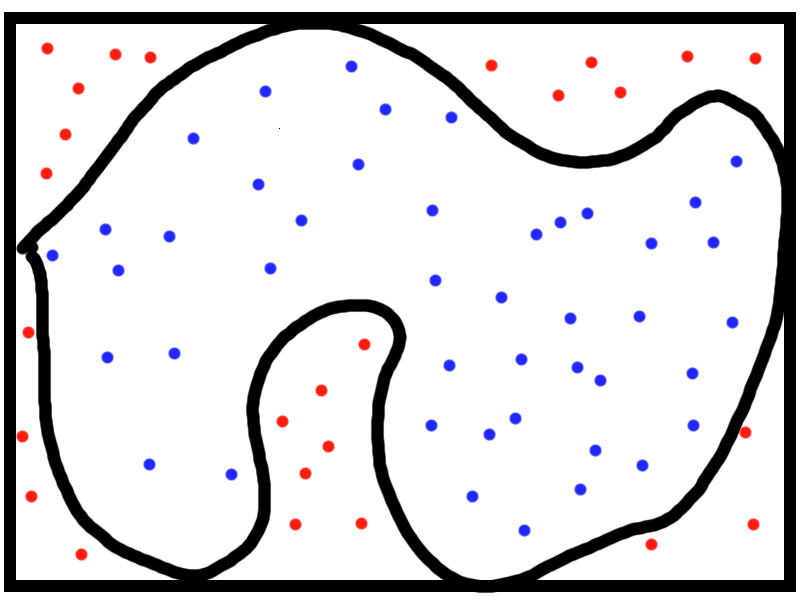
\includegraphics[width = .5\textwidth]{montecarloex.png}
    \caption{Monte Carlo method for area estimation.}
    \label{fig:mcarea}
\end{figure}

We will see later in the paper that the concept of random sampling in order to estimate a distribution is thematically similar to the above example of randomly sampling to estimate a parameter. Just like how we can use sample moments to estimate moments of a random variable, we can use samples to estimate the entire distribution. That is, we can use complicated sampling algorithms to find a sample estimate of the PDF or PMF of a random variable. We do this using Markov Chains, hence the name \emph{Markov Chain Monte Carlo}.

\section{Bayesian Inference}

\label{section:bayesian}

This introduction to basic Bayesian formulation and terminology comes from the first chapter of \emph{Bayesian Data Analysis} by Gelman et al \cite{gelman}. In this setting, we are interested in making statistical conclusions about parameters $\theta$ or future data $\widetilde{y}$. First, we start with the assumption that $\theta$ is not some fixed unknown value but has a distribution. We can make probabilistic statements about $\theta$ conditioned on observed values $y$. We use the following notation, where lowercase $p$ refers to the probability density function (PDF) or probability mass function (PMF) of a distribution:
$p(\cdot | \cdot)$ represents a conditional density function and $p(\cdot)$ represents a marginal density function.

To begin conditioning $\theta$ on $y$, we must start with a \emph{model}, a joint distribution of $\theta$ and $y$. Once this is given, we can write the following from the definition of conditional probability:
\[p(\theta , y) = p(\theta) p(y| \theta),\]
where $p(\theta)$ is called the \emph{prior distribution} and $p(y| \theta)$ is called the \emph{sampling distribution}. The \emph{posterior} distribution $p(\theta|y)$ is given by Bayes theorem:
\[p(\theta |y) = \frac{p(\theta) p(y| \theta)}{p(y)}.\]

An important aspect of the posterior distribution that will remain relevant in our discussion of MCMC is that the denominator is a constant with respect to $\theta$ since the posterior is conditional on $y$. This means that the posterior distribution is proportional to the joint distribution of $\theta$ and $y$, written as $p(\theta|y)\propto p(\theta , y) = p(\theta) p(y| \theta)$, where $\propto$ is read as ``proportional to''. As we will see in the next section, this makes the Metropolis-Hastings algorithm a powerful tool for estimating complicated posterior distributions.

\begin{exmp}[Beta binomial conjugacy]
    One of the simplest closed form posterior distributions we can describe is $p(x|\theta)$ with $x\sim$ Bin$(n,\theta)$ with $\theta \sim$ Beta$(\alpha,\beta)$ as a prior. Suppose that we observe one value $x$. By Bayes' theorem we get \begin{align*}
        p(\theta|x)&=\frac{p(x|\theta)p(\theta)}{p(x)}\\
        &\propto p(x|\theta)p(\theta) \quad \text{(Denominator is a constant w.r.t. $\theta$)}\\
        &={n \choose x}\theta^x(1-\theta)^{n-x}\frac{\theta^{\alpha-1}(1-\theta)^{\beta-1}}{B(\alpha,\beta)}\\
        \intertext{Where $B(\alpha,\beta)=\frac{\Gamma(\alpha)\Gamma(\beta)}{\Gamma(\alpha+\beta)}$ and $\Gamma(x)=\int_0^\infty t^{x-1}e^{-t}dt$. The $B$ function normalizes the beta PDF $\theta^{x+\alpha-1}(1-\theta)^{n-x+\beta-1}$.}
    \end{align*}
    
    The final term shows us that the posterior has a Beta$(\alpha+x,\beta+n-x)$ distribution.
\end{exmp}

In this example we see how for some simple distributions a conjugacy arises where we get simple closed forms for posterior distributions given certain priors. The next example serves to illustrate other ways that a posterior might have a simple closed form. Later, we will revisit it to show an extension where the posterior has no simple closed form.

\begin{exmp}[Hardy-Weinberg equilibrium \cite{stephens}]
    Consider a population where every individual has a pair of genes that are each one of the alleles $A$ and $a$. Let $r$ be the frequency of $A$ in the population. We are interested in modeling $r$ since the frequency of alleles may tell us more about a population than the counts of certain phenotypes will. We assume that the population is sufficiently large, no mutations occur, and the individuals mate randomly within their generation. These are our model assumptions, but it should be noted that they are not realistic conditions (populations can be small, mutations do occur, and mating is driven by complicated relationships that are not random). \emph{Hardy-Weinberg equilibrium} tells us that for every generation after the first generation of random mating, the frequencies of $AA$, $Aa$ and $aa$ are $r^2$, $2r(1-r)$ and $(1-r)^2$ respectively \cite[p.~207]{ross}\cite[p.~35]{gen}. We use the word `equilibrium' because once entered, the genotype proportions will remain the same for each subsequent generation. Let $x$ be a 3-tuple of counts of each genotype observed, with $x=(n_{AA},n_{Aa},n_{aa})$, with each $n$ being a number of observed individuals. The Hardy-Weinberg equilibrium proportions of each genotype describe a multinomial distribution for $p(x|r)$. Consider the problem where we observe counts of certain genotypes in a population and are interested in modeling $r$. We assign $r$ an \emph{uninformative prior} with $r\sim \text{Unif}(0,1)$. We can find the posterior distribution as
    \begin{align*}
        p(r|x)&=\frac{p(x|r)p(r)}{p(x)}\\
        &\propto r^{2n_{AA}} (2r(1-r))^{n_{Aa}} (1-r)^{2n_{aa}}\\
        &\propto r^{2n_{AA}+n_{Aa}}(1-r)^{2n_{aa}+n_{Aa}}.
    \end{align*}
    
    This tells us that the posterior is distributed Beta$(2n_{AA}+n_{Aa}+1,2n_{aa}+n_{Aa}+1)$.
\end{exmp}

% Another concept that will be central to some of the examples given in this paper is the \emph{directed acyclic graph} (DAG) \cite[p.~82]{causal}. We can use DAGs to represent conditional dependencies between different variables in our model drawn with arrows. For example, consider the following DAG:

% \[\text{Temperature} \rightarrow \text{Weather forecast} \rightarrow \text{Taking a coat}\]

% If the temperature is low on a given day, a meteorologist might say that the forecast is ``chilly''. This in turn might might make a listener decide to take a coat when they leave their house. These conditional dependencies are shown in the above graph. If we condition on the forecast, then knowing the temperature does not change the probability of taking a coat. Thus we can say that Taking a coat is conditionally independent of the temperature given the forecast.

\section{Metropolis-Hastings Algorithm}

Among the many methods that fall under the term Markov Chain Monte Carlo, the Metropolis-Hastings algorithm\cite{blitzstein}\cite{mcmc}\cite{gelman} is one of the most popular and influential. The algorithm is an adaptation of a random walk (example 2.10) that constructs a Markov chain whose stationary distribution is the desired distribution. With just the knowledge of what the desired distribution is \emph{proportional} to, we can use the Metropolis-Hastings algorithm to sample from that distribution. This makes the Metropolis-Hastings algorithm particularly useful in Bayesian inference, where the joint distribution may be easier to find than the posterior. To begin, we define the \emph{Metropolis algorithm}.

\subsection{Metropolis Algorithm}

\begin{defn}[{Metropolis algorithm}]
    Let $p(x)$ be a desired stationary distribution. Let $J(\cdot|\cdot)$ be a \emph{proposal distribution}, also called a \emph{jumping distribution}. The Metropolis algorithm requires that $J$ have the special property of being \emph{symmetric}: it must satisfy $J(x|y)=J(y|x)$ for all $x,y$. We can construct the desired Markov chain $X_0, X_1,...$ according to the following algorithm:


\begin{enumerate}
    \item Initialize $X_0=x_0$ where $p(x_0)>0$. This choice can be made randomly or deterministically. 
    \item At any step $t\geq 1$ with $X_t=x_t$, sample proposal $x^*$ from $J(x^*|x_t)$.
    \item Calculate the \emph{Metropolis ratio}
    \[r(x_t,x^*)=\frac{p(x^*)}{p(x_t)}.\]
    \item Calculate the acceptance probability
    \[a(x_t,x^*)=\min(r(x_t,x^*),1).\]
    \item Transition to new state with the following probabilities \[X_{t+1}=\begin{cases}x^*, & \text{with probability }a(x_t,x^*) \\
    x_t, & \text{with probability }1-a(x_t,x^*)
    \end{cases}\]
\end{enumerate}
\end{defn}

To interpret this algorithm, we can think of it as a random walk that chases the mode of a distribution. When $p(x^*)>p(x_t)$, we know that $x^*$ has a higher chance of occurring that $x_t$. In this case, $r(x_t,x^*)>1$ and $a(x_t,x^*)=1$. So the chain transitions to $x^*$ with probability 1. If $p(x^*)<p(x_t)$, then the chain only transitions to $x^*$ with probability $a(x_t, x^*)=r(x_t, x^*)<1$. Intuitively, the chain spends more time at and ``chases'' modes.

One of the most important aspects of the Metropolis algorithm is step (4). The Metropolis ratio is a measure of the relative probabilities (or densities in the continuous state space case) of different states. Since it is a ratio of the same probability mass function (PMF) or probability density function (PDF), any normalizing constants cancel out. This makes the Metropolis algorithm particularly useful in a Bayesian setting for sampling from complicated posterior distributions. 

We can show that the stationary distribution of the Metropolis chain exists and is the desired distribution $p(x)$ \cite[p.~279]{gelman}. 
\begin{proof}
    We know that a Markov Chain that is aperiodic and irreducible has a stationary distribution. We know that the Metropolis chain is aperiodic since it is always possible to transition from a state back to itself in any number of steps that could be coprime with each other. In particular it is possible that $x^*=x_t$. As long as our proposal distribution has a positive probability for every state in the state space, then we can say that the chain is irreducible: there is some positive probability that every state will be proposed and then a positive probability that it will be accepted.
    
    To show that the stationary distribution is $p(x)$, we check that the chain is reversible with respect to $p$ by checking if $(X_k, X_{k+1})$ and $(X_{k+1}, X_k)$ have the same distribution. Suppose without loss of generality $p(x_a)\leq p(x_b)$. In this case, the Metropolis ratio $r(x_a, x_b)=\frac{p(x_b)}{p(x_a)}>1$ and $a(x_a,x_b)=1$ consequently. We have 
    \begin{align*}
        p(X_{t} =x_a , X_{t+1} =x_b )&= p(X_{t+1}=x_b|X_t=x_a)p(X_t=x_a)\\
        &=p(X_t=x_a)\cdot J(x_b|x_a) \cdot a(x_a,x_b)\\
        &=p(x_a)J(x_b |x_a ).
    \end{align*}
    
    That is, the joint probability of observing states $x_a$ and $x_b$ in a row is equal to the probability of observing $x_a$ and then proposing $x_b$. Since $p(x_a)\leq p(x_b)$, we know that $X_{t+1}=x_b$ will be automatically accepted. Now consider the reverse distribution:
    \begin{align*}
        p(X_{t} &=x_b , X_{t+1} =x_a ) = p(X_t=x_b)p(X_{t+1}=x_a|X_t=x_b) \\
        &=p(X_t=x_b)\cdot J(x_a|x_b)\cdot a(x_b,x_a)\\
        &=p(x_b)J(x_a |x_b )\frac{p(x_a)}{p(x_b)} \\
        &=p(x_a)J(x_a |x_b )\\
        &=p(x_a)J(x_b |x_a ) \quad \text{($J(\cdot|\cdot)$ is symmetric)}
    \end{align*}
    
    The first line is that the joint probability of observing $x_b$ and $x_a$ in a row is the the probability of observing $x_b$, proposing $x_a$, and then accepting $x_a$. This simplifies, and then using the requirement that $J$ be symmetric, we achieve the reversibility condition.
    
\end{proof}

Note that this proof only applies to sampling from discrete distributions. The Metropolis-Hastings algorithm still works for continuous distributions. A measure-theoretic proof can be found in \cite{measure}.

\medskip

Here is a simple example of how to apply the Metropolis algorithm.

\begin{exmp}[Sampling from a Beta distribution]
\label{ex:betamh}
    The Metropolis algorithm allows us to sample from a distribution for which only an unnormalized PDF is known. The Beta PDF with parameters $\alpha, \beta$ is given by 
    \[f_{\text{Beta}}(x|\alpha, \beta) = \frac{x^{\alpha-1}(1-x)^{\beta -1}}{B(\alpha, \beta)},\]
    where $B(\alpha, \beta)$ is a normalizing constant. We know what this normalizing constant is, but supposing that we did not know it we could still use the Metropolis algorithm to sample from the Beta distribution. For this example we will simulate sampling from a Beta(2,~6) distribution. The steps are as follows:
    \begin{enumerate}
        \item First, Initialize $X_0$ as some number $x_0$. This can be done in many ways, but for this example we sample from a Uniform(0,~1) distribution. 
        \item At step $t$ where $X_t=x_t$, sample a proposal state $x^*$ from the Uniform(0,~1) distribution, i.e. $J(x^*|\cdot) \sim Unif (0,1)$. The choice of distribution here is normally a strategic choice but for this example we use the uniform distribution for simplicity. Notice that this choice satisfies the symmetric condition.
        \item Compute the Hastings ratio using the unnormalized Beta PDF:
        \[r(x_t,x^*)=\frac{x^{*^{2-1}}(1-x^*)^{6 -1}}{x_t^{2-1}(1-x_t)^{6 -1}}.\]
        \item Calculate the acceptance probability: \[a(x_t,x^*)=\min(r(x_t,x^*),1).\]
    \item Transition to state $x^*$ with probability $a(x_t,x^*)$, otherwise transition to same state $x_t$. 
    \end{enumerate}
    
    The results of this simulation are shown in figure \ref{fig:betamh}. The figure shows that our algorithm did a pretty good job of sampling from the true distribution. The R code for this simulation can be found in the appendix.
    
    \begin{figure}
    
  
  \centering
    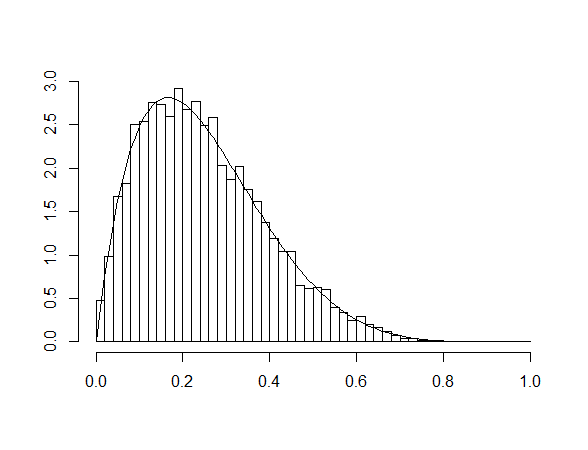
\includegraphics[width=.65\textwidth]{NEWbetahm.png}
    \caption{Histogram of results from using M-H to sample from Beta(2,6). $10^4$ interations. True density superimposed.}
    \label{fig:betamh}
\end{figure}
    
    
\end{exmp}

\subsection{Metropolis Hastings}
The algorithm that is in common use today is the Metropolis-Hastings algorithm\cite[p.~279]{gelman}. With the Metropolis-Hastings alrogithm, $J$ is no longer required to be symmetric and the Metropolis ratio is replaced with the \emph{Hastings ratio}:
\[r(x_t,x^*) =
\frac{p(x^*)/J(x^*|x_t)}
{p(x_t)/J(x_t |x^*)}.\]

\begin{defn}[{Metropolis-Hastings algorithm}]
    Let $p(x)$ be a desired stationary distribution. Let $J(\cdot|\cdot)$ be a \emph{proposal distribution}, also called a \emph{jumping distribution}. We no longer require $J$ to be symmetric, just that $J(x|a)>0$ for all $x,a$ in the support of $p(x)$. We can construct the desired Markov chain $X_0, X_1,...$ according to the algorithm:


\begin{enumerate}
    \item Initialize $X_0=x_0$ where $p(x_0)>0$. This choice can be made randomly or deterministically. 
    \item At any step $t\geq 1$ with $X_t=x_t$, sample proposal $x^*$ from $J(x^*|x_t)$.
    \item Calculate the \emph{Metropolis-Hastings ratio}
    \[r(x_t,x^*) =
\frac{p(x^*)/J(x^*|x_t)}
{p(x_t)/J(x_t |x^*)}.\]
    \item Calculate the acceptance probability
    \[a(x_t,x^*)=\min(r(x_t,x^*),1).\]
    \item Transition to new state with the following probabilities \[X_{t+1}=\begin{cases}x^*, & \text{with probability }a(x_t,x^*) \\
    x_t, & \text{with probability }1-a(x_t,x^*)
    \end{cases}\]
\end{enumerate}
\end{defn}

The proof of stationarity follows almost exactly the same as with the Metropolis algorithm: the lack of a symmetric jumping distribution is corrected for in the Hastings ratio \cite[p.~498]{blitzstein}. The benefit of the Metropolis-Hastings algorithm is that we now have more freedom for our choice of $J$. This means that we could potentially make choices that will lead to faster convergence of our simulation.

The next example shows us how the choice of sampling method can make a difference. It is brought up now but will be revisited again later.
\begin{figure}[H]
  %\centering
    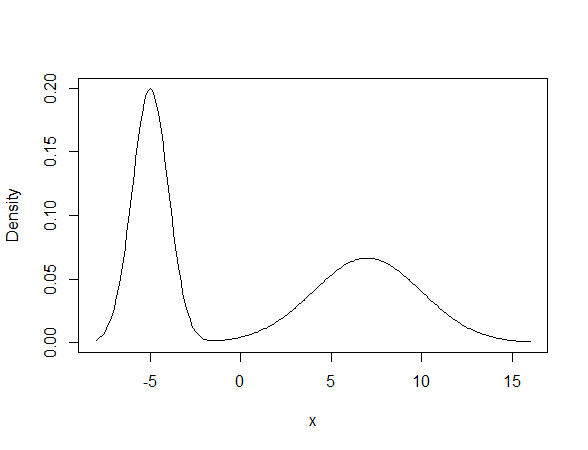
\includegraphics[width = .5\textwidth]{mixdensity.png}
    \caption{Density function for mixture of two normals.}
    \label{fig:mix}
\end{figure}
\begin{exmp}[Sampling from a mixture of normals]
\label{ex:mixture}
    Let $f_i(x)$ be the PDF for N$(\mu_i,~\sigma_i^2)$. Consider the distribution given by the following PDF: $f(x)=\pi f_1(x)+ (1-\pi)f_2(x)$. This distribution is called a {\em mixture of two normals}. It means that each point is drawn from one of two normal distributions and the probabilities of coming from each distribution are $\pi$ and $1-\pi$. This distribution does not necessarily have a single local maxima. For example, figure \ref{fig:mix} shows the PDF of a mixture of N$(-5,~1)$ and N$(7,~3)$ with $\pi=0.5$.
    
    Is the Metropolis algorithm able to sample from this distribution as easily as it did for the Beta example? We apply the Metropolis algorithm with $J(x^*|x_t)\sim \text{N}(x_t, 0.5^2)$. This jumping distribution is symmetric because the Normal distribution is symmetric about its mean. Below are the result from running the simulation four times:

    In this example each simulation was initialized at -1 and run for $10^5$ iterations. As we can see, the histograms significantly deviate from the true density curve in each example. In this case the Metropolis algorithm shows some shortcomings. We will revisit this example in a later section when we talk about diagnostics for our simulations.
    
    Code for this simulation is provided in the appendix. The code is written to allow for experimenting with simulating other distributions and using other proposal distributions easily.
    
        \begin{figure}[h]
        \centering
        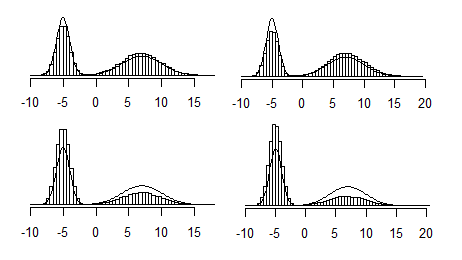
\includegraphics[width = 5 in]{bigger4ex.png}
        \caption{Side by side histograms for 4 instances of the Metropolis-Hastings simulation in example \ref{ex:mixture}.}
        \label{fig:4way}
    \end{figure}
\end{exmp}


In the next example I make reference to a problem where there is no closed form posterior distribution available. This is an example where MCMC sampling necessary out of practicality, as there is no closed form for the posterior distribution.

\begin{exmp}[{Hardy-Weinberg extension with inbreeding coefficient \cite{stephens}}]
\label{ex:hwinbreedingmh}
    As explained before, the basic assumption of Hardy-Weinberg equilibrium is that mating is perfectly random. We can extend the problem by introducing an inbreeding coefficient $f\in [0,1]$. The interpretation of $f$ is the probability that an individual will have two of the same allele that are identical by descent (IBD) \cite[p.~64]{gen}. Put simply, an individual that is IBD is a homozygote that inherited the same allele twice from the one recent ancestor shared by both parents. See figure \ref{fig:IBD}. We are interested in finding the population frequency of IBD, $f$, because if we count the number of $A$ alleles in the population without accounting for IBD individuals, we will overestimate the frequency of $A$ alleles in the population. If an individual's alleles are inherited independently and not due to inbreeding, then probabilities of each of the three genotypes follows from the original Hardy-Weinberg equilibrium. On the other hand, if the two alleles are IBD, then the genotype frequency is simply the allele frequency, i.e., $p(AA|IBD)=r$, $p(aa|IBD)=1-r$ and $p(Aa|IBD)=0$. This is because we know that the individual is a homozygote, so knowing one allele tells us the other. Thus the frequencies of $AA$, $Aa$, and $aa$ are $fr+(1-f)r^2$, $(1-f)2r(1-r)$, and $f(1-r)+(1-f)(1-r)^2$ respectively \cite[p.~65]{gen}. That is because
    
    \[p(AA)=p(IBD)p(AA|IBD)+p(not~ IBD)p(AA| not~IBD)=fr+(1-f)r^2.\]
    
    The $p(Aa)$ and $p(aa)$ values can be calculated similarly. Now the problem is that given a tuple of observations $x=(n_{AA},n_{Aa},n_{aa})$ we would like to find the joint posterior of $f$ and $r$ conditioned on $x$. If we assign uninformative uniform priors to $f$ and $r$ we get
    \begin{align*}
        &p(f,r|x)\propto \\ &\left[fr+(1-f)r^2\right]^{n_{AA}}\left[(1-f)2r(1-r)\right]^{n_{Aa}} \left[f(1-r)+(1-f)(1-r)^2\right]^{n_{aa}}
    \end{align*}
    
    \begin{figure}
        \centering
        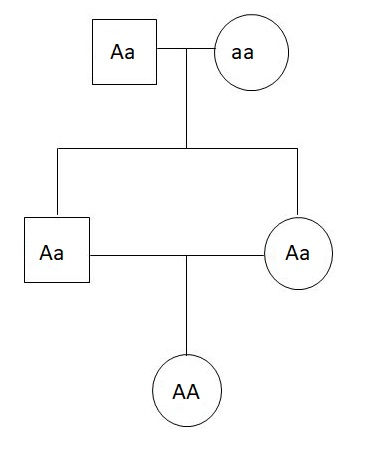
\includegraphics[width = .5\textwidth]{IBD.jpg}
        \caption{The descendent here is IBD. It is a homozygote where each allele is from the same ancestor. We are interested in modeling the occurrences of $A$ in {\em non-inbred} individuals, so counting both alleles here would be an overestimate.}
        \label{fig:IBD}
    \end{figure}
    
    Given observed $x$, the exact posterior distribution could be found by taking the double integral of the numerator of the posterior. However, the closed form for the posterior for any arbitrary $x$ is not easy to find. Therefore MCMC sampling is an appealing alternative. From the above we have enough information to begin applying the Metropolis algorithm. Say we observe $x=(50, 21, 29)$. We choose a jumping distribution of sampling $f$ and $r$ each from the Unif$(0,1)$ distribution. The following result in figure \ref{fig:inbreedmh} shows results after $10^4$ iterations.
    
    \begin{figure}
        \centering
        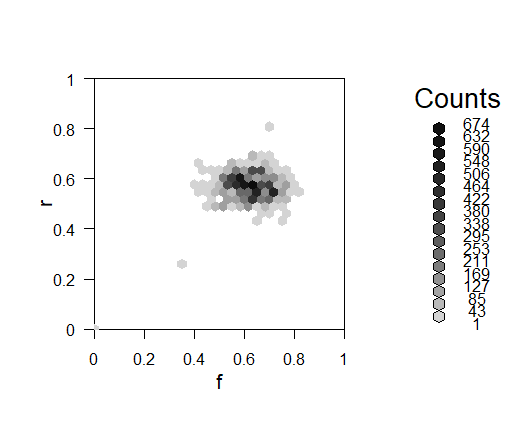
\includegraphics[width=4 in]{inbreed.png}
        \caption{Two way histogram for results of $p(f,r)$ using the Metropolis-Hastings algorithm described in example \ref{ex:hwinbreedingmh}. Made using the hexbin package for R, see the appendix.}
        \label{fig:inbreedmh}
    \end{figure}
    
    This image can be understood as a two way histogram, or a heat map. The two axes represent values of $f$ and $r$. Darker colors of the histogram represent high frequencies of observing those values. In this way the historgram serves as a Probability Mass Function (PMF) estimate for the joint distribution $p(f,r)$.
    
\end{exmp}

\section{Gibbs Sampling}

The second tool to cover in the MCMC toolbox is {\em Gibbs sampling}\cite[p.~508]{blitzstein}\cite[p.~276]{gelman}, an algorithm that allows for sampling from joint distributions of any dimension. The basic concept is that we can iteratively sample from conditional distributions of one random variable conditioned on the remaining random variables. In practice, Gibbs sampling and the Metropolis-Hastings algorithm can be used as building blocks for more complicated algorithms.

\begin{defn}[{Gibbs sampler \cite[p.~508]{blitzstein}\cite[p.~24]{mcmc}\cite[p.~276]{gelman}}]
    
    We wish to sample from the joint distribution $p(\theta_1,...,\theta_d)$.
    
    
    \begin{enumerate}
    \item Initialize our vectors of values $(\theta_1,...,\theta_d)$ either randomly or deterministically. 
    \item At time $t$, we sample from each component conditioned on the \emph{current} values of all the other components. That is, for the $i$th component we sample from $p(\theta_i|\theta_1^t,...,\theta_{i-1}^t, \theta_{i+1}^{t-1}, ..., \theta_d^{t-1})$, where the subscript indexes the component of the joint distribution and the superscript indexes the timestamp that the current value was sampled at.  
    
\end{enumerate}

The description above describes sampling from each conditional in order. The process is called a {\em systemic scan Gibbs sampler}. We could also sample randomly from each conditional distribution. In this case, the process is called a {\em random scan Gibbs sampler}.
    
\end{defn}

We can revisit an earlier example and use Gibbs sampling to explore the Beta Binomial conjugacy. In this example we can see how to use conditional distributions to sample from a joint distribution, and how this naturally extends into sampling from a marginal distribution.


\begin{exmp}[{Beta-Binomial conjugacy with Gibbs sampling \cite{gibbs}}]
\label{ex:gibbsex}
In this example, suppose we are interested in sampling from a joint distribution $p(\cdot,\cdot)$ given by 
\[p(x,\mathbf{p}) \propto {n \choose x} \mathbf{p}^{x+\alpha-1}(1-\mathbf{p})^{n-x+\beta-1},\]
where $x\in \N$, $x \leq n$, $\mathbf{p} \in [0,1]$, and $n, \alpha, \beta$ are all known. While it may not be obvious how to sample directly from this joint distribution, the conditional distributions $p(x|\mathbf{p})$ and $p(\mathbf{p}|x)$ have clear interpretations with $p(x|\mathbf{p})\sim$ Binomial $(n,\mathbf{p})$ and $p(\mathbf{p}|x)\sim$ Beta $(x+\alpha,n-x+\beta)$. We can use these conditional distributions to sample from the joint. Here we implement systemic scan Gibbs sampler. First, we initialize $\mathbf{p}_0$ as some number, either randomly or deterministically. Next we sample $x_0$ from $p(x_0|\mathbf{p}_0)\sim Bin(n, \mathbf{p}_0)$. Then we sample $\mathbf{p}_1$ from $p(\mathbf{p}_1|x_0)\sim Beta(x_0+\alpha, n-x_0+\beta)$. We continue going through the systemic scan of $X$ and $\mathbf{p}$ for $N$ iterations until we get our resulting chain:
\[p_0, x_0, p_1, x_1, ..., p_N, x_N.\]

\begin{figure*}
        \centering
        \begin{subfigure}[b]{0.475\textwidth}
            \centering
            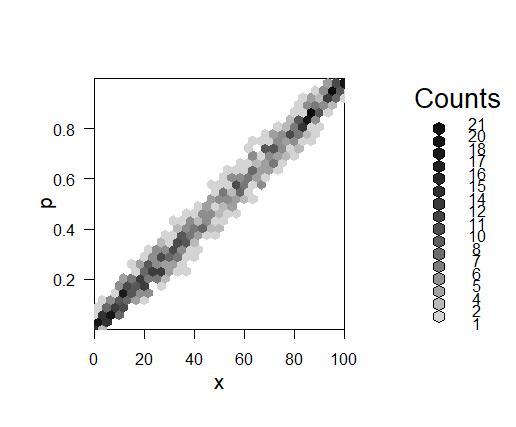
\includegraphics[width=\textwidth]{bettergibbsEX.png}
            \caption{Two-way histogram, darker is higher density. Note the dark spot in the lower left.}    
            \label{fig:exex}
        \end{subfigure}
        \hfill
        \begin{subfigure}[b]{0.475\textwidth}  
            \centering 
            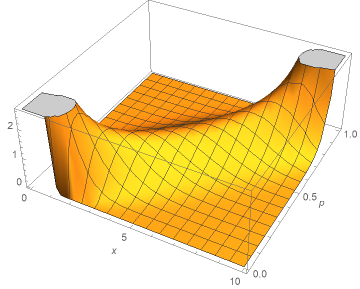
\includegraphics[width=\textwidth]{download5.png}
            \caption{3D plot of ${n \choose x} \mathbf{p}^{x+\alpha-1}(1-\mathbf{p})^{n-x+\beta-1}$. Note this is not a density as it is missing its normalizing constant.}    
            \label{fig:download}
        \end{subfigure}
        \caption{Gibbs sampling result for example  \ref{ex:gibbsex} compared to true density.} 
        \label{fig:gibbsex}
    \end{figure*}

\end{exmp}

This is effectively a sampling from $p(x,\mathbf{p})$. The histogram for the result of this Gibbs sampler can be seen in figure \ref{fig:exex}. Code is supplied in the appendix. Interestingly, if we ignore all of the $p_i$, what is left is an effective sample from the marginal distribution $p(x)$. The (very rough) intuition for this comes from the concept of Monte Carlo simulation in section 3. The marginal distribution $p(x)$ is given by
\[p(x) = \int p(x,\mathbf{p}) d\mathbf{p},\]
that is, the marginal is the joint with the other variable integrated out. Our Gibbs sampler provides us with samples of $X$ from the conditional distribution $p(x|\mathbf{p})$ for many different values of $\mathbf{p}$. This is the sampling counterpart to integrating over all values of $\mathbf{p}$, which is why we should believe that that Gibbs sampler for the marginal does converge to the true marginal.

\begin{exmp}[{Hardy-Weinberg with inbreeding using Gibbs \cite{stephens}}]

\label{ex:inbreedinggibbs}

Gibbs sampling provides a natural alternative to the Metropolis-Hastings approach to the Hardy-Weinberg with inbreeding problem. We will see in the next section that it even produces a more desirable result. Since we wish to sample from the joint posterior of $p(f,r)$ conditioned on our data, we have a natural multivariate candidate for our Gibbs sampling algorithm. However, for this particular problem it helps to consider our data as a list of individuals instead of a list of counts. The simulation is aided by introducing a \emph{latent variable} for each individual. In Bayesian modeling, a latent variable is an unobserved variable that is assumed to cause our data. In this case we have $Z_i$ indicating whether or not the $i$th individual is inbred by decent (IBD). I use $G_i$ to represent the genotype of the $i$th individual, with $G$ being the vector of all $G_i$ (the same goes for $Z$ and $Z_i$). For the sake of calculations and notation, we also introduce the following variables that are functions of the previous variables: We have $U=\sum Z_i$, the total number of IBD individuals. We have $Y_1$ is the number of $A$ alleles in non-IBD individuals. There are $2(n-U)$ alleles in non-IDB individuals to look at, so $Y_1 \sim Bin (2(n-U), r)$. We have $Y_2$ is the number of $AA$ IBD individuals. We count these differently because we want $AA$ to count as 1 for IDB individuals. Note that $Y_2 \sim Bin (U, r)$. Let $Y=Y_1+Y_2$. So $Y$ can be interpreted as a count of the occurrences of $A$ with the IBD $AA$ individuals counting as 1. We note the following pieces of information:
\[Z_i \sim Bernoulli(f)\]
\[p(G_i=AA | Z_i=1,r) = r,\quad p(G_i=AA | Z_i=0,r) = r^2\]
\[p(G_i=Aa | Z_i = 1,r)= 0, \quad p(G_i=Aa | Z_i=0,r) = 2r(1-r)\]
\[p(G_i=aa | Z_i = 1,r) = (1-r), \quad p(G_i =aa | Z_i=0,r) = (1-r)^2\]
\[U\sim Binomial(n,f), \quad  Y_1 \sim Binomial(2(n-U), r), \quad Y_2 \sim Binomial(U, r)\]
\[Y \sim Binomial(2n-U, r)\]


We use the following Gibbs sampler:
\begin{enumerate}
    \item Initialize $f,r$ with their starting values. We assign a uniform prior of $Beta(1,1)$ to each.
    \item Sample from $p(Z|G_i,f,r)$. This gives us simulated values of whether each individual is IBD.
    \item Sample from $p(f,r|Z)$. This is the original problem, but with the help of our latent variable $Z$ in our Gibbs sampler, we are able to break this up into two steps:
        \begin{enumerate}
            \item Sample from $p(f|Z)$. It is the same to sample from $p(f|U)$.
            \item Sample from $p(r|Z)$. It is the same to sample from $p(r|Y)$.
        \end{enumerate}
    \item Repeat steps 2 and 3 for many iterations.
\end{enumerate}

\begin{figure}[h]
    \centering
    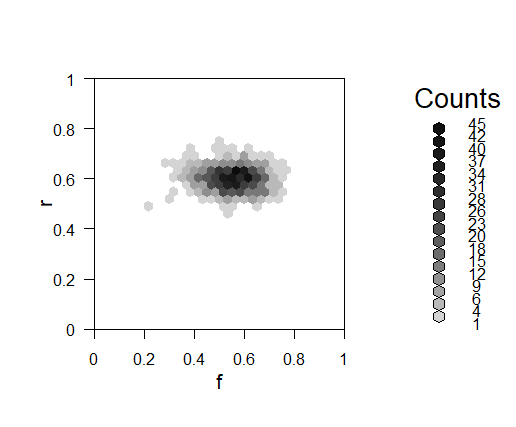
\includegraphics[width= .75\textwidth]{gibbsinbreeding1.png}
    \caption{Two way histogram for results of $p(f,r)$ using the Gibbs sampler described in example \ref{ex:inbreedinggibbs}.}
    \label{fig:inbreedinggibbs}
\end{figure}

The substitutions we make in steps 3a and 3b are backed up by some logical intuition. In the case of this model, we know that $f$ is conditionally independent of $Z$ given $U$ and that $r$ is conditionally independent of $Z$ given $Y$.


Let us show that we can sample from each of these conditional distributions. First, in step 2 we have that $p(Z|G_i,f,r)$ is a Bernoulli distribution whose paramaters we now compute. We have that
\begin{align*}
&p(Z_i = 1 | G_i = AA, r, f) =\\
&\frac{p(G_i=AA|Z_i=1, f, r) ~p(Z_i=1|f, r)}{p(G_i=AA|Z_i=0, f, r)~p(Z_i=0|f, r) + p(G_i=AA|Z_i=1, f, r)~p(Z_i=1|f, r)}\\
\intertext{Note that further conditioning $p(G_i=AA|Z_i=1, r)$ on $f$ provides no new information, so we can safely remove it from the term. The same goes for the second term and removing $r$:}
&=\frac{p(G_i=AA|Z_i=1, r) ~p(Z_i=1|f)}{p(G_i=AA|Z_i=0, r)~p(Z_i=0|f) + p(G_i=AA|Z_i=1, r)~p(Z_i=1|f)}\\
&= \frac{fr}{(1-f)r^2 + fr}.
\end{align*}

Similarly, for $G_i=aa$ we have $p(Z_i = 1 | G_i = aa, r, f)=\frac{f(1-r)}{(1-f)(1-r)^2+f(1-r)}$. We also know that $p(Z_i=1|G_i=Aa)=0$, since IBD implies homozygous. Now we have our Bernoulli proportions for the full conditional distribution of $Z_i$.

To sample from $p(f|U)$ and $p(r|Y)$, we make use of the Beta-Binomial conjugacy from example 4.1. As noted above, $U$ and $Y$ are each binomially distributed. Using the Beta priors assigned to $f$ and $r$, the Beta-Binomial conjugacy allows us to sample from the conditional distributions. We have that $p(f|U)\sim Beta(1+U, 1+(n-U))$ and $p(r|Y)\sim Beta(1+Y, 1+((2n-U)-Y))$.

We now have all the steps for our Gibbs sampler and can implement it in R. The results for running the simulation for $10^4$ iterations are displayed in figure \ref{fig:inbreedinggibbs}. The code is included in the appendix.

Note that this result has more or less the same mode as our previous result in exampled \ref{ex:hwinbreedingmh}, which suggests that both methods worked as intended. The distributions are different, which shows differences between the methods. We can see in figure \ref{fig:inbreedinggibbs} that the result is relatively smooth. This difference is discussed in further detail in the next section.
\end{exmp}

\section{Diagnostics for Simulations}

We have so far outlined the mathematical foundations for the construction of MCMC sampling algorithms. This section deals with the different diagnostic tools that tell us about the efficiency and representativeness of our simulations. Examples will show how different simulations will affect our diagnostics.

One of the most basic visual tools is a {\em trace plot}\cite[p.179]{dogs}. This plot is simply a graph of the chain values as a function of the number of steps. We can superimpose several MCMC simulations on one trace plot in order to get an idea of the convergence of our simulation. In example \ref{ex:mixture} we looked at sampling from a mixture of normals. There we saw evidence that the simulation might not have converged properly in $10^3$ iterations. Figure \ref{fig:mixtrace} shows the superimposed trace plots of 3 trials of the simulation in example \ref{ex:mixture}.

In this example, it appears that one of the chains favored the left side mixture component while the other two chains favored the right component. The trace plot shows that the different chains favor different modes, thus not generating a representative sample from the distribution within 1000 steps. Asymptotically, we know that our chain will have the desired stationary distribution, but we do not have evidence that we are getting the desired samples within 1000 steps. We can try again using $10^4$ steps instead as show in figure \ref{fig:mixlong}. Still we have similar behavior. Doing more iterations than this starts to become lengthy.

    \begin{figure*}
        \centering
        \begin{subfigure}[b]{0.475\textwidth}
            \centering
            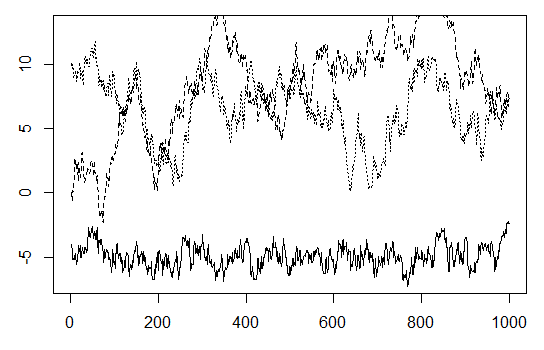
\includegraphics[width=\textwidth]{mixtrace.png}
            \caption{$J(x^*|x_t)\sim \text{N}(x_t, 0.5^2)$\newline n=$10^3$}    
            \label{fig:mixtrace}
        \end{subfigure}
        \hfill
        \begin{subfigure}[b]{0.475\textwidth}  
            \centering 
            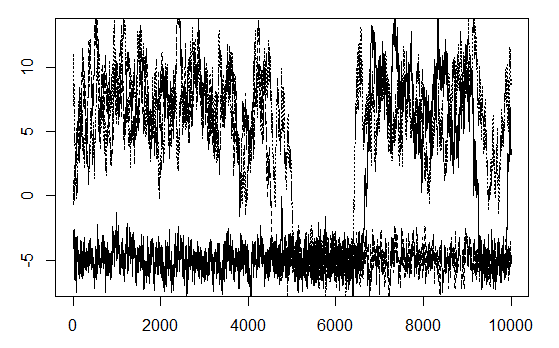
\includegraphics[width=\textwidth]{longmixture.png}
            \caption{$J(x^*|x_t)\sim \text{N}(x_t, 0.5^2)$\newline n=$10^4$}    
            \label{fig:mixlong}
        \end{subfigure}
        %\vskip\baselineskip
        \begin{subfigure}[b]{0.475\textwidth}   
            \centering 
            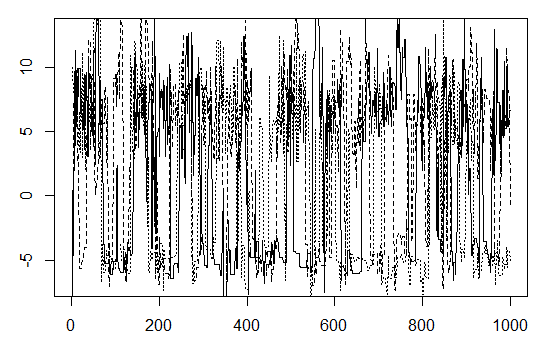
\includegraphics[width=\textwidth]{bettermixing.png}
            \caption{$J(x^*|x_t)\sim \text{N}(x_t, 3^2)$\newline n=$10^3$}    
            \label{fig:mixbetter}
        \end{subfigure}
        \quad
        \begin{subfigure}[b]{0.475\textwidth}   
            \centering 
            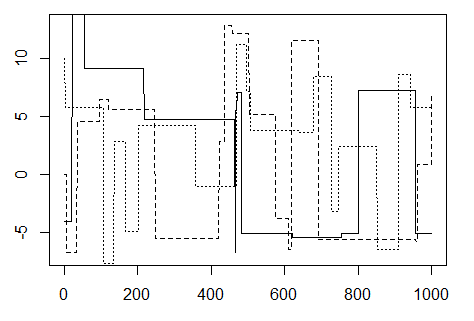
\includegraphics[width=\textwidth]{mixbad.png}
            \caption{$J(x^*|x_t)\sim \text{N}(x_t, 300^2)$\newline n=$10^3$}    
            \label{fig:mixbad}
        \end{subfigure}
        \caption{Trace plots for variations of the experiment done in example \ref{ex:mixture}.} 
        \label{fig:traceplots}
    \end{figure*}

Intuitively, we should note that this distribution is not well suited for Metropolis-Hastings sampling. Recall that we interpreted the Metropolis-Hastings algorithm as ``chasing modes''. Given two modes, we can see from the trace plots that the chain tends to get stuck in one mode. However, recall that in the original example the proposal distribution we used was N$(x_t,0.5^2)$. By increasing the variance from $0.5^2$, we increase the probability of proposing points closer to the other mode. If we increase the variance of the proposal distribution, we see better evidence of convergence in our trace plot. Let's try using N$(x_t,3^2)$ instead. The results in figure \ref{fig:mixbetter} show no obvious separations of our trace plots. This gives us stronger evidence for convergence.

It might be tempting to therefore conclude that have a high variance proposal distribution is always better. This is not the case. If we increase the variance to $300^2$, we can see in figure \ref{fig:mixbad} that our chains get stuck at a handful of points. Because the proposal distribution has such high variance, the proposed points have very low density. This means that the chain does not frequently transition between states. In practice, the variance of the proposal distribution should be neither too small nor too large.

Additionally, we can learn about burn-in from these trace plots. Since we initialize our chains with some value, the values of the chain will be influenced by this choice. To mitigate the influence of the initial value, we can discard some number of the first samples. Trace plots give us a visual for deciding this burn-in cut off. Consider for example where we used the Metropolis algorithm to sample from the Beta(2,6) distribution.

\begin{figure}[h]
    \centering
    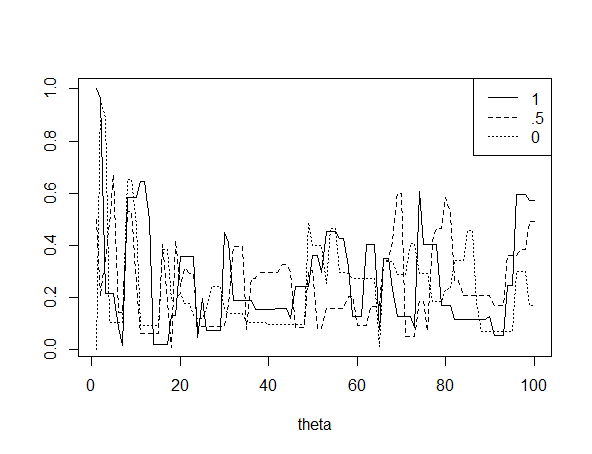
\includegraphics[width= .75\textwidth]{betamixturestarts.png}
    %\caption{Two way histogram for results of $p(f,p)$ using the Gibbs sampler described in example \ref{ex:inbreedinggibbs}.}
    \label{fig:betamixstarts}
\end{figure}

In this plot we run the same simulation three times, sampling from the Beta(2,6) distribution using the Metropolis algorithm. The legend shows the starting points of the chains. We can see that all three plots move away from the early values at about 10 steps in. In this case, we can see a burn-in of about 10 steps.

One of the most basic numerical diagnostics for MCMC simulation is the \emph{autocorrelation function}. This idea is used in time series analysis. The following definition comes in part from an econometrics textbook.

\begin{defn}[{Autocorrelation function \cite[p.~182]{dogs} \cite[p.~532]{stock}}]

The autocorrelation function (ACF) is a function of a Markov chain $X_1,... X_n$ and a number of lags $k$. The autcorrelation at lag $k$, $ACF(k)$ is the correlation of $(X_t, X_{t-k})$.
\[ACF(k)=\frac{cov(X_t, X_{t-k})}{\sqrt{var(X_t)var(X_{t-k})}}.\]

\end{defn}

This gives us one scalar number. The autocorrelation function is the autocorrelation as a function of lags. We interpret autocorrelation as an approximation of independence. We would like our simulated sample to have the property of being $n$ independent samples. Since we are dealing with Markov chains, we know that sample $i+1$ is necessarily dependent on sample $i$. So it is impossible to have a truly independent sample. However, a sample with low autocorrelation will show that the effect of this dependency has been minimized for the purpose of sampling from the stationary distribution. 

Consider the following example where we examine the ACF for $r$ in the inbreeding problem using the Metropolis-Hastings algorithm from example \ref{ex:hwinbreedingmh}.

\begin{figure}[h]
    \centering
    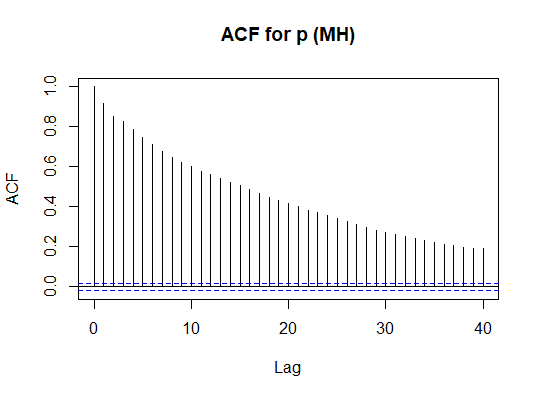
\includegraphics[width= .65\textwidth]{ACFpMH.png}
    \caption{The ACF for $r$ using the Metropolis-Hastings algorithm in example \ref{ex:hwinbreedingmh}.}
    \label{fig:ACFpMH}
\end{figure}

We can see that the autocorrelation is decreasing, but it is doing so at a very slow rate. We can compare this to the ACF for $r$ when using the Gibbs sampler, as seen in figure \ref{fig:ACFpGibbs}.


\begin{figure}[h]
    \centering
    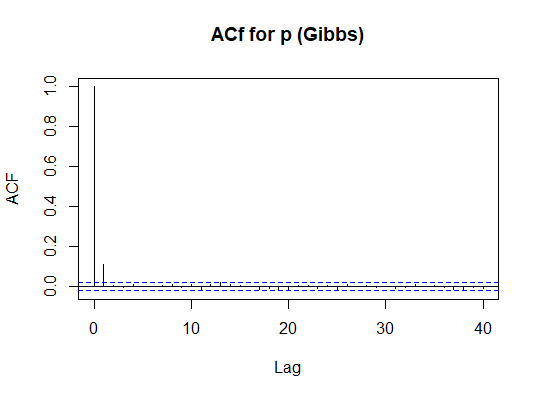
\includegraphics[width= .65\textwidth]{ACFpGibbs.png}
    \caption{The ACF for $r$ using the Gibbs sampler in example \ref{ex:inbreedinggibbs}.}
    \label{fig:ACFpGibbs}
\end{figure}
    
Here our result has a much lower ACF than with the Metropolis-Hastings algorithm. We therefore expect or simulation to \emph{mix} quicker. That is, simulate independent samples quicker. We care about our samples having little dependence on each other. We come up with a measure of our number of independent samples as follows.

    \begin{defn}[{Effective sample size \cite[p.~184]{dogs}}]
    
    The effective sample size (ESS) attempts to estimate how many sufficiently independent samples we have from our simulation. Given a Markov chain simulation, the ESS is defined as
    \[ESS = N \left / \left(1+2\sum_{k=1}^{\infty}ACF(k)\right) \right.\]
    
    In practice, the infinite sum may be stopped when $ACF(k) < 0.05$, as the ACF typically decreases with $k$ \cite[p.~184]{dogs}.
    
    \end{defn}
    
    Software packages provide implementations for these functions. For simulating $r$ in the inbreeding problem, with $N=1,000$ we can see that the Metropolis-Hastings simulations yielded an ESS of 271.724. On the other hand, our Gibbs sampler yields an ESS of approximately 759.715.
    
    \section{Discussion and Future Work}
    

    This paper provides a basic outline of the fundamentals of MCMC simulation, with consideration given to the theoretical basis. In total, this paper gives the foundations for carrying out examples of the Metropolis-Hastings algorithm, Gibbs sampling, and illustrative examples that explain the theoretical underpinnings. The provided code in the appendix allows for readers to recreate all of the simulations and experiments on their own. The code can be easily modified to conduct new experiments. 
    

    In section \ref{section:bayesian} we introduced the concept of a bayesian posterior distribution. It was noted that the denominator for the posterior in Bayes' Theorem is a constant, thus making the Metropolis-Hastings algorithm practical for sampling from intractable Bayesian posteriors. With the inbreeding problem, this came in handy since there is no closed form solution for the posterior. One benefit to using the Metropolis-Hastings Algorithm to sample from the posterior was that it was easy to set up. We simply chose suitable proposal distributions and were able to get informative samples of $r$. This paper did not examine the impact of different proposal distributions on the simulation results, but the results shown in figure \ref{fig:traceplots} tell us about what considerations we can make. Given the apparent better performance of the Gibbs sampler on this example, there may have been room for improvement by choosing different proposal distributions.
    
    In the inbreeding example, the Gibbs sampler appears to have supplied a better simulation of $p(r)$, as evident by the ACF in figure \ref{fig:ACFpGibbs} and the higher ESS value. The math to motivate our simulation was much more difficult and complex. However, we did not rely on a proposal distribution for our simulation, thus making the simulation design easier. 
    
    If we would like to draw conclusions about $f$ and $r$, one option is to examine the modes of the distribution $p(f,r)$. Both methods found modes around $0.6$ for both $r$ and $f$. This tells us that given the data $n_{AA}=50$, $n_{Aa}=21$, $n_{aa}=29$, $r$ can be estimated as approximately $0.6$, and the same with $f$. In both cases there was an ovular shape to the distribution histogram, showing that there was more variance in $f$ samples than in the $r$ samples. This makes some sense, as the inbreeding rate is a little difficult to gleam from the genotype count data.
    
    
    The biggest challenge in MCMC simulation is getting independent results. As I have shown, it is not too difficult to get samples from the distributions we examined. The Metropolis-Hastings algorithm is not too difficult to design  and implement, but knowing that our result is converging to the desired distribution in a timely manner is an open question. There is no way to detect this with any certainty. One popular method to insure greater independence in sampling is \emph{Hamiltonian Monte Carlo simulation}, a type of MCMC simulation that incorporates Hamiltonian particle dynamics to make samples more random while still being theoretically sound. Just like knowing a densitty function down to a constant tells us the relative densities of different points, it can also tell us about the gradient of the density function. This is additional useful for drawing samples. \cite{mcmc} is very detailed in this regard.
    
    There are summaries of how MCMC is used in different fields in \cite{mcmc} and \cite{rev}. In particular, \cite{rev} gives citations for best uses of MCMC methods in the fields of chemistry and biology, as well as a fun exmaple with prison code cracking. In addition, there are best practices to explore. For example, MCMC simulation is not easily parallelizable, since sampling from Markov chains depends on earlier results. One parallelization approach is to run many short chains instead of one long chain in order to get many independent results. \cite{mcmc} recommends this as best practice, but further research could investigate why this is the case.
    

\begin{thebibliography}{9}


\bibitem{blitzstein} J.K.~Blitzstein and J. Hwang, {\em Introduction to Probability}, 2nd ed. CRC Press, Boca Raton FL, 2019.

\bibitem{mcmc} S. Brooks, et al., eds., {\em Handbook of markov chain monte carlo}, Chapman and Hall/CRC, London UK, 2011.

\bibitem{gibbs} G. Casella and E. I. George, \emph{Explaining the Gibbs sampler}, The American Statistician \textbf{46.3} (1992), 167-174.

\bibitem{measure} S. Chib and E. Greenberg, {\em Understanding the Metropolis-Hastings Algorithm}, The American Statistician \textbf{49.4} (1995), 327-335.

\bibitem{gen} J.~Crow and M.~Kimura, {\em An Introduction to Population Genetics Theory}. Harper and Row, 1970.

\bibitem{rev} P. Diaconis, {\em The markov chain monte carlo revolution}. Bulletin of the American Mathematical Society \textbf{46.2} (2009), 179-205.

\bibitem{gelman} A. Gelman, et al., {\em Bayesian Data Analysis} 3rd ed. Chapman and Hall/CRC, London UK, 2013.
 

\bibitem{dogs} J. Kruschke, {\em Doing Bayesian data analysis: A tutorial with R, JAGS, and Stan}, Academic Press, Cambridge MA, 2014.

\bibitem{causal} J. Peters, et al. {\em Elements of causal inference: foundations and learning algorithms}. MIT press, Cambridge MA, 2017.

\bibitem{pierre} B. Pierre, {\em Markov chains: Gibbs fields, Monte Carlo simulation, and queues}, Vol. 31. Springer-Verlag, New York NY, 1991.

%\bibitem{rosenthal} J. Rosenthal, {\em A first look at rigorous probability theory}, 2nd ed. Springer-Verlag, New York NY, 1991.

\bibitem{ross} S. Ross, {\em Introduction to Probability Models}, 9th ed. Academic Press, Cambridge MA, 2007.

\bibitem{stephens} M. Stephens. Simple Examples of Metropolis–Hastings Algorithm https://stephens999.github.io/fiveMinuteStats/MH-examples1.html (visited December 5, 2019)

\bibitem{stock} J. Stock and M. Watson, {\em Introduction to Econometrics}, Vol. 3. Pearson, Boston MA, 2012.



\end{thebibliography}

\newpage

\section{Appendix: R code for examples}

For the 2 variable histogram plots in this paper I used the hexbin package for R, version 1.28.0.

\medskip

Example \ref{ex:betamh}.\begin{verbatim}
#This function returns the function for our unormalized Beta PDF.
betakern=function(x, alpha, beta){
  return(x^(alpha-1)*(1-x)^(beta-1))
}

mh = function(alpha, beta, niter, init=NA){
  theta=rep(0, niter)
  #By default, the chain is initialized from a uniform distribution.
  if(is.na(init)){
    theta[1] <- runif(1)
  }
  #You can also specify an inital value.
  else{
    theta[1]=init
  }
  for (i in 2:niter){
    #Propose new value.
    theta.p <- runif(1)
    #Calculate ratio.
    r <- betakern(theta.p, alpha, beta)/betakern(theta[i-1], alpha, beta)
    #Sample from Bernoulli(acceptance probability).
    flip <- rbinom(1,1,min(r,1))
    theta[i] <- if(flip==1) theta.p else theta[i-1]
  }
  return(theta)
}
    \end{verbatim}
    
Example \ref{ex:mixture}. \begin{verbatim}
Metropolis <- function(F_sample # R function for 
                                # distribution we want to sample from
               , y0 # initializing value
               , F_prop  # proposal distribution
               , niter=1e5   # iterations
){
  y = rep(0,niter)
  y[1] = y0    # starting location for random walk
  accepted = rep(0,niter-1)
  
  for(i in 2:niter)    {
    # Sample from proposal distribution.
    y.p <- F_prop(y[i-1])

    R=F_sample(y.p)/F_sample(y[i-1])
    
    a <- rbinom(1,1,min(R, 1))
    if(a){
      y[i] = y.p
      accepted[i-1] = 1
    }    
    else{
      y[i] = y[i-1]
    }    
  }
  return(list(y, accepted))
}

sample_dist = function(x){.5*dnorm(x,-5,1)+.5*dnorm(x,7,3)}
y0 = -1
prop_dist = function(x){rnorm(1, x, sqrt(0.5) )}
result = Metropolis(sample_dist, y0, prop_dist)
    \end{verbatim}
    
    
Example \ref{ex:hwinbreedingmh}. \begin{verbatim}
# Likelihood function for Hardy-Weinberg model with inbreeding.
# n1, n2, n3 refer to nAA, nAa, naa respectively.
inblike = function(n1,n2,n3,f,r){
    return((f*r+(1-r)*r^2)^n1*((1-f)*2*r*(1-r))^n2 *(f*(1-r)+(1-f)*(1-r))^n3)
}

# Metropolis-Hastings algorithm applied to Hardy-Weinberg with inbreeding.
inbreeding = function(n1=50, n2=21, n3=29, niter=10000){
  f=rep(0, niter)
  r=rep(0, niter)
  f[1] <- 0
  r[1] <- 0
  for (i in 2:niter){
    f.p <- runif(1)
    r.p <- runif(1)
    ratio <- inblike(n1,n2,n3,f.p,r.p)/inblike(n1,n2,n3,f[i-1],r[i-1])
    flip <- rbinom(1,1,min(ratio,1))
    if(flip==1){
      f[i]=f.p
      r[i]=r.p
    }
    else{
      f[i]=f[i-1]
      r[i]=r[i-1]
    }
  }
  return(list(f=f,r=r))
}
\end{verbatim}

Example \ref{ex:gibbsex} \begin{verbatim}
ex=function(n=100, a=0, b=0, N=1000){
  p=rep(0,N)
  x=rep(0,N)
  p[1]=runif(1)
  x[1]=rbinom(1, n, p[1])
  for(i in 2:N){
    p[i]=rbeta(1, x[i-1]+a, n-x[i-1]+b)
    x[i]=rbinom(1, n, p[i])
  }
  return(data.frame(x=x, p=p))
}
\end{verbatim}

Example \ref{ex:inbreedinggibbs}. \begin{verbatim}
gibbsinbreeding <- function(ndata=c(50,21,29), 
                       prior = c(1, 1, 1, 1), 
                       init = c(.2, .5), 
                       N = 1000) {
  
  # Represent data as individual observations.
  obs_data <- rep(c("AA", "Aa", "aa"), times = ndata)
  obs_data <- factor(obs_data, levels = c("AA", "Aa", "aa"))

  f <- r <- rep(0, N)
  f[1] <- init[1]
  r[1] <- init[2]
  for (i in 2:N) {
    # Calculate p(Z|f,p) for each case of gi:
    z_probs <- ifelse(obs_data == "AA", 
    f[i-1] * r[i-1] / (f[i-1] * r[i-1] + (1 - f[i-1]) * r[i-1] ^ 2),
               ifelse(obs_data == "Aa", 0,
               ifelse(obs_data == "aa",
               f[i-1] * (1 - r[i-1]) / 
               (f[i-1] * (1 - r[i-1]) + (1 - f[i-1]) * (1 - r[i-1]) ^ 2), NA))) 
    
    z <- runif(n = length(z_probs)) < z_probs
    z_counts <- table(z)
    
    f[i] <- rbeta(n = 1, 
    shape1 = z_counts[2] + prior[1], shape2 = z_counts[1] + prior[2])
    
    nz_genos <- table(obs_data[z == FALSE])
    
    nz_A = 2 * nz_genos["AA"] + nz_genos["Aa"] 
    nz_a = 2 * nz_genos["aa"] + nz_genos["Aa"]
    
    z_genos <- table(obs_data[z == TRUE])
    z_A = z_genos["AA"]
    z_a = z_genos["aa"]
    
    r[i] <- rbeta(n = 1,
    shape1 = prior[3] + nz_A + z_A, shape2 = prior[4] + nz_a + z_a)
  }
  return(data.frame(f=f,r=r))
}
\end{verbatim}

\end{document}

